\chapter{sensitive sequencer} 
\label{sec:sequencer}
\lstset{style=6502Style}
\lstset{ 
   aboveskip=5pt,
   belowskip=0pt,
}

\begin{definition}[Jeffrey Says\index{Jeffrey Says}]
\setlength{\intextsep}{0pt}%
\setlength{\columnsep}{3pt}%
\begin{wrapfigure}{l}{0.12\textwidth}

\includegraphics[width=\linewidth]{src/callout/psych.png} 
\end{wrapfigure}
\small
Programming is as for the Burst Generators, but you have the
freedom of 255 steps allowed played back at varying speeds via the
Sequencer Speed control. You can leave the program mode in two
ways: press SPACE, and next time you go back in with SHIFT-Q the
stuff you already defined is not cleared and you add to the end of it,
or press RETURN, and next time you go in the sequencer is cleared.
Use the SPACE option to change pattern in mid-sequence, for
example, or to ‘see how it looks so far’.
\end{definition}

A sequencer is just a pretend person, gaily twiddling new patterns at different positions on the screen. Instead of painting pixels
the boring way with one's bare hands we can program a whole bunch of pretend user input and let Psychedelia play it for us. In order
to see how this works in practice, let's look at how the sequencer data is loaded and processed by walking through the sequencer
that comes packaged with Psychedelia. Before that, we can take a look at it in all its glory on the next page along with the less
glorious looking data structure that is responsible for it.

\clearpage                                                                 
\begin{figure}[H]                                                          
    \centering                                                             
    \hspace*{1cm}
    \begin{adjustbox}{width=17cm,center}                                   
      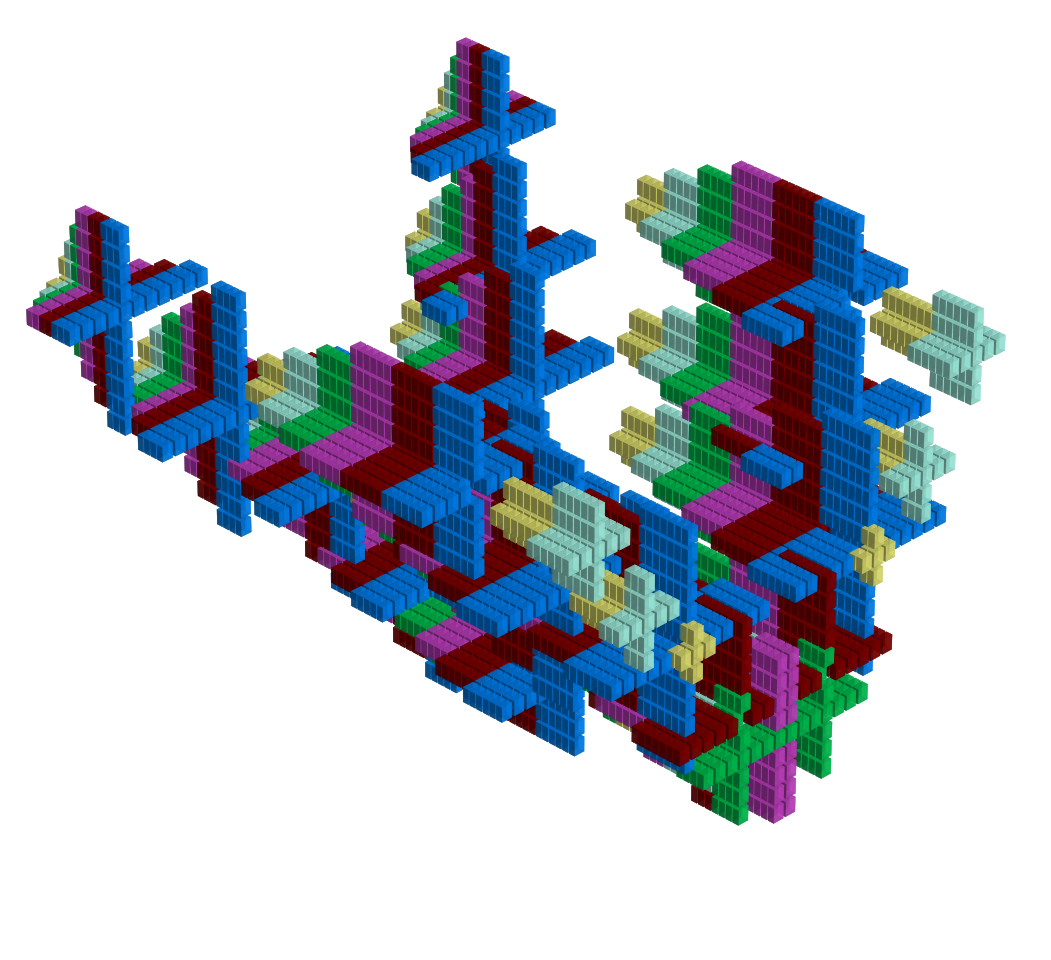
\includegraphics[width=14cm]{src/sequencer/pattern0-45.png}%           
    \end{adjustbox}                                                        
\caption{Evolution of the Default Sequencer.}                                           
\end{figure}                                                               
\clearpage                                                                 
                                                                           
\begin{lstlisting}[basicstyle=\ttfamily\scriptsize,caption=Sequencer definition in \icode{sequencer\_data.asm}.,escapechar=\%]
sequencerDataStorage = $C300
  ; currentSymmetrySetting%\index{currentSymmetrySetting}%: 'Current symmetry setting.'                     
  ; Possible values are 0 - 4:                                              
  ; 'NO SYMMETRY     '                                                      
  ; 'Y-AXIS SYMMETRY '                                                      
  ; 'X-Y SYMMETRY    '                                                      
  ; 'X-AXIS SYMMETRY '                                                      
  ; 'QUAD SYMMETRY   '                                                      
  .BYTE $01          ; Y-Axis Symmetry

  ; smoothingDelay%\index{smoothingDelay}%: 'Because of the time taken to draw larger patterns speed
  ; increase/decrease is not linear. You can adjust the compensating delay
  ; which often smooths out jerky patterns. Can be used just for special FX)
  ; though. Suck it and see.'                                               
  .BYTE $0B

  ; Sequencer Position 1
  .BYTE $04,$04;  ; X/Y Co-ordinates: X/Y Position (absolute position).   
  .BYTE PULSAR;   ; Index to pattern in pixelXPositionHi/LoPtrArray   

  ; Sequencer Position 2
  .BYTE $08,$09;  ; X/Y Co-ordinates: X/Y Position (absolute position).   
  .BYTE PULSAR;   ; Index to pattern in pixelXPositionHi/LoPtrArray   

  ; Sequencer Position 3
  .BYTE $0C,$0C;  ; X/Y Co-ordinates: X/Y Position (absolute position).   
  .BYTE PULSAR;   ; Index to pattern in pixelXPositionHi/LoPtrArray   

  ; Sequencer Position 4
  .BYTE $10,$11;  ; X/Y Co-ordinates: X/Y Position (absolute position).   
  .BYTE PULSAR;   ; Index to pattern in pixelXPositionHi/LoPtrArray   

  ; Sequencer Position 5
  .BYTE $14,$13;  ; X/Y Co-ordinates: X/Y Position (absolute position).   
  .BYTE PULSAR;   ; Index to pattern in pixelXPositionHi/LoPtrArray   

  ; Sequencer Position 6
  .BYTE $17,$13;  ; X/Y Co-ordinates: X/Y Position (absolute position).   
  .BYTE PULSAR;   ; Index to pattern in pixelXPositionHi/LoPtrArray   

  ; Sequencer Position 7
  .BYTE $FF,$01;  ; X/Y Co-ordinates: X/Y Position (absolute position).   
  .BYTE MULTICROSS ; Index to pattern in pixelXPositionHi/LoPtrArray   

  ; Sequencer Position 8
  .BYTE $41,$FF;  ; X/Y Co-ordinates: X/Y Position (absolute position).   
  .BYTE $00;;  ; Index to pattern in pixelXPositionHi/LoPtrArray   

  ; Sequencer Position 9
  .BYTE $06,$01;  ; X/Y Co-ordinates: X/Y Position (absolute position).   
  .BYTE MULTICROSS ; Index to pattern in pixelXPositionHi/LoPtrArray   

  ...
  ; Sequencer Position 254
  .BYTE $FF,$80;  ; X/Y Co-ordinates: X/Y Position (absolute position).   
  .BYTE $EE;;  ; Index to pattern in pixelXPositionHi/LoPtrArray   

  ; Sequencer Position 255
  .BYTE $FD,$FF;  ; X/Y Co-ordinates: X/Y Position (absolute position).   
  .BYTE $FF;;  ; Index to pattern in pixelXPositionHi/LoPtrArray   
    
\end{lstlisting}

\clearpage
\rhead[]{\icode{MaybeQPressed}}
\textbf{Lines 1440-1457. \icode{\textbf{MaybeQPressed\index{MaybeQPressed}}}}
\begin{lstlisting}[escapechar=\%]
MaybeQPressed%\index{MaybeQPressed}%    
        CMP #KEY_Q ; Q pressed?
        BNE MaybeVPressed

        ; Q was pressed. Toggle the sequencer on or off.
        LDA sequencerActive%\index{sequencerActive}%
        BNE TurnSequenceOff

TurnSequenceOn
        LDA #SEQUENCER_ACTIVE
        STA currentVariableMode%\index{currentVariableMode}%
        JMP ActivateSequencer%\index{ActivateSequencer}%
        ;Returns

        ;Turn the sequencer off.
TurnSequenceOff   
        LDA #$00
        STA sequencerActive%\index{sequencerActive}%
        STA stepsRemainingInSequencerSequence%\index{stepsRemainingInSequencerSequence}%
        JMP DisplaySequencerState%\index{DisplaySequencerState}%
\end{lstlisting}
\textbf{Lines 2558-2575. \icode{\textbf{ActivateSequencer\index{ActivateSequencer}}}}
\begin{lstlisting}[escapechar=\%]
ActivateSequencer%\index{ActivateSequencer}% 
        LDA #>sequencerDataStorage
        STA currentSequencePtrHi%\index{currentSequencePtrHi}%

        LDA #<sequencerDataStorage
        STA currentSequencePtrLo%\index{currentSequencePtrLo}%

        LDA #$FF
        STA sequencerActive%\index{sequencerActive}%

        LDA shiftPressed%\index{shiftPressed}%
        AND #$01
        BNE ShiftPressedSoProgramSequencer

        ; Start Playing the Sequencer
        LDA sequencerSpeed%\index{sequencerSpeed}%
        STA stepsRemainingInSequencerSequence%\index{stepsRemainingInSequencerSequence}%

        LDA #$00
        STA currentVariableMode%\index{currentVariableMode}%

        JSR DisplaySequencerState%\index{DisplaySequencerState}%
        RTS 
\end{lstlisting}
\clearpage

\textbf{Lines 1440-1457. \icode{\textbf{MaybeOPressed}}:} To see the sequencer in action we have to activate it. Pressing \icode{Q} turns it on or off, depending on whether
it is already, um, on or off. This is where we make this important decision so it seems like a good place to start in our effort to understand how the thing works.

 \icode{sequencerActive\index{sequencerActive}} is the variable that keeps track of on- and off-ness. Anyway if it's on: we turn it off
with \icode{TurnSequenceOff}. If it's off however: we do something much more exciting. We turn it on with the grandly titled routine
\icode{ActivateSequencer\index{ActivateSequencer}}, which we come to next. Programming is fascinating and complex I find.

\textbf{Lines 2558-2575. \icode{\textbf{ActivateSequencer\index{ActivateSequencer}}}:}  Despite its heady name, this routine just sets a couple of variables.
Storing \icode{\$FF} in \icode{sequencerActive\index{sequencerActive}} flags that the sequencer is active, which as we just saw is useful to know if the player wants
to turn it off by pressing \icode{Q} again. 

There are a couple of other meaningful things to do in here. One is to set up the interval at which we will feed data into the sequencer.
This is managed by \icode{steps\-Remaining\-In\-SequencerSequence}. We'll see how this is used in the very next page. The value we initialize it
with is itself a user-definable setting called \icode{sequencerSpeed\index{sequencerSpeed}}.

The final bit to do is to store the location of the sequencer data in a pair of variables that we will use to read in the sequencer data. We
saw this technique used in the previous chapter on Burst data. The high and low bytes of the address \icode{sequencerDataStorage} (which is \icode{\$C300}) are loaded to 
\icode{currentSequencePtrHi\index{currentSequencePtrHi}} (which gets \icode{\$C3}) and \icode{current\-SequencePtrLo} (which gets \icode{\$00}) respectively:
\begin{lstlisting}[escapechar=\%]
        LDA #>sequencerDataStorage
        STA currentSequencePtrHi%\index{currentSequencePtrHi}%

        LDA #<sequencerDataStorage
        STA currentSequencePtrLo%\index{currentSequencePtrLo}%
\end{lstlisting}

With that, we can consider the Sequencer fully activated. Psychedelia is now ready to use it in a way that you might find slightly 
convoluted, or even moderately interesting. Read on.

\clearpage


\rhead[]{\icode{MainInterruptHandler}}
\textbf{Lines 728-743. \icode{\textbf{MainInterruptHandler}}}
\begin{lstlisting}[escapechar=\%]
MainInterruptHandler
        ; The sequencer is played by the interrupt handler.
        ; Check if it's active.
        LDA stepsRemainingInSequencerSequence%\index{stepsRemainingInSequencerSequence}%
        BEQ SequencerNotActiveCheckJoystickInput%\index{SequencerNotActiveCheckJoystickInput}%
        DEC stepsRemainingInSequencerSequence%\index{stepsRemainingInSequencerSequence}%
        BNE SequencerNotActiveCheckJoystickInput%\index{SequencerNotActiveCheckJoystickInput}%

        ; If the sequencer is active we'll end up here and
        ; load the sequencer data so that it can be played.
        LDA sequencerSpeed%\index{sequencerSpeed}%
        STA stepsRemainingInSequencerSequence%\index{stepsRemainingInSequencerSequence}%
        JSR LoadDataForSequencer%\index{LoadDataForSequencer}%
\end{lstlisting}

\clearpage

\textbf{Lines 728-743. \icode{\textbf{MainInterruptHandler}}:} We already encountered the operation of the \icode{MainInterruptHandler} 
\hyperref[sec:listing_commentary]{\textcolor{blue}{ our walk through of the listing.}}. What we have here is the first part of the same routine
that shipped with the commercial version of Psychedelia. It is pretty much the same in principle: it looks for input from the user on the joystick
and moves the cursor around in response, and it also keeps the buffers fed: the buffers being the arrays that tell Psychedelia what to paint and where.

Normally this would be based on the user input, but if we have a sequencer active then this is also our opportunity to feed those buffers with data from 
the sequencer, over and over. As we mentioned at the head of the chapter, the Sequencer is just like a pre-programmed bit of user input fed repeatedly
into the Psychedelia engine, over and over, until you make it stop. 

So since \icode{MainInterruptHandler} is the place where actual user input is processed it makes sense that it is also the place where 'simulated' user
input such as that from the sequencer data is also digested.

All we do in this little section is determine whether we want to process some of the sequencer data or not. This is where the variable \icode{stepsRemainingInSequencerSequence\index{stepsRemainingInSequencerSequence}}
we intialized on the previous page comes in. If it's zero the sequencer isn't active and we can just jump straight to \icode{SequencerNotActiveCheckJoystickInput\index{SequencerNotActiveCheckJoystickInput}}. Otherwise
we decrement it by one. If it's still not zero, then we also skip loading any sequencer data. However if it has reached the magic number of zero it's time to chew some of the 
goodness in \icode{sequencerDataStorage}. First we reinitialize \icode{stepsRemainingInSequencerSequence\index{stepsRemainingInSequencerSequence}} to the selected sequencer speed so it won't be zero the next time
around. That done we are ready to process us some sequencer data by calling \icode{LoadDataForSequencer\index{LoadDataForSequencer}}. Let's go to the next page and see what does. (I wonder what!)

\clearpage
\rhead[]{\icode{LoadDataForSequencer}}
\textbf{Lines 2616-2663. \icode{\textbf{LoadDataForSequencer\index{LoadDataForSequencer}}}}
\begin{lstlisting}[escapechar=\%]
LoadDataForSequencer%\index{LoadDataForSequencer}%   
        INC currentStepCount%\index{currentStepCount}%
        LDA currentStepCount%\index{currentStepCount}%
        CMP bufferLength%\index{bufferLength}%
        BNE MaybeLoadSequencerDataToCurrentSlot

        LDA #$00
        STA currentStepCount%\index{currentStepCount}%

MaybeLoadSequencerDataToCurrentSlot   
        TAX 
        LDA currentIndexForCurrentStepArray,X
        CMP #$FF
        BEQ LoadValuesFromSequencerData

        LDA shouldDrawCursor
        AND trackingActivated%\index{trackingActivated}%
        BEQ MoveToNextPositionInSequencer%\index{MoveToNextPositionInSequencer}%

        TAX 
        LDA currentIndexForCurrentStepArray,X
        CMP #$FF
        BNE MoveToNextPositionInSequencer%\index{MoveToNextPositionInSequencer}%

LoadValuesFromSequencerData   
        LDY #$02
        LDA (currentSequencePtrLo%\index{currentSequencePtrLo}%),Y
        CMP #$C0
        BEQ MoveToNextPositionInSequencer%\index{MoveToNextPositionInSequencer}%

        LDA baseLevel%\index{baseLevel}%
        STA currentIndexForCurrentStepArray,X

        LDA sequencerDataStorage + $01
        STA initialSmoothingDelayForStep,X
        STA smoothingDelayForStep,X

        LDA sequencerDataStorage
        STA symmetrySettingForStepCount%\index{symmetrySettingForStepCount}%,X

        LDY #$02
        LDA (currentSequencePtrLo%\index{currentSequencePtrLo}%),Y
        STA pixelXPositionArray%\index{pixelXPositionArray}%,X

        INY 
        LDA (currentSequencePtrLo%\index{currentSequencePtrLo}%),Y
        STA pixelYPositionArray%\index{pixelYPositionArray}%,X

        INY 
        LDA (currentSequencePtrLo%\index{currentSequencePtrLo}%),Y
        STA patternIndexArray%\index{patternIndexArray}%,X

\end{lstlisting}

\clearpage

\textbf{Lines 2616-2663. \icode{\textbf{LoadDataForSequencer\index{LoadDataForSequencer}}}:} We've already seen a version of this movie before. When we loaded the burst data in the previous chapter
our routine was parsing the data piece by piece and loading it into the buffers. We're doing the same thing here. The only difference is that instead of doing it just
the once (and loading all of it in one go), for a burst, we're calling this routine a few times every second from \icode{MainInterruptHandler}. The exact frequency was controlled on the previous page
by \icode{stepsRemainingInSequencerSequence\index{stepsRemainingInSequencerSequence}}. 

Since we're being called at least a few times every second we're not attempting to read all of the sequencer data at once here like we did for the bursts. Instead we just read in the next step in
the sequence and add that to the buffers. Once that's done, we advance our pointer (\icode{currentSequencePtrLo\index{currentSequencePtrLo}}) a few bytes so that it is in the correct position the next time we're called.

Each step is three bytes long. The first step we load in, the first time we're called, is this guy:

\begin{lstlisting}[escapechar=\%]
  ; Sequencer Position 1
  .BYTE $04,$04;  ; X/Y Co-ordinates: X/Y Position (absolute position).   
  .BYTE PULSAR;   ; Index to pattern in pixelXPositionHi/LoPtrArray   
\end{lstlisting}

\textbf{Lines 2625-2637. \icode{\textbf{MaybeLoadSequencerDataToCurrentSlot}}:} Is there a free spot in the buffers for some of our sequence data or not? If yes, great: we can jump to \icode{LoadValuesFromSequencerData}.
Otherwise we just move our pointer \icode{currentSequence\-PtrLo} to the next three bytes in the sequencer data and bail out by calling \icode{MoveTo\-NextPosition\-InSequencer}. 

\textbf{Lines 2639-2663. \icode{\textbf{LoadValuesFromSequencerData}}:}  I don't know, maybe we should like, load some data? The first two bytes are taken from the very top of the sequencer data every time:
\begin{lstlisting}[escapechar=\%]
sequencerDataStorage = $C300
  .BYTE Y_AXIS_SYMMETRY          ; Y-Axis Symmetry
  .BYTE $0B                      ; Smoothing Delay
\end{lstlisting}
We load them like so the appropriate position in the \icode{initialSmoothingDelayForStep} and \icode{symmetrySettingForStepCount\index{symmetrySettingForStepCount}} buffers like so:
\begin{lstlisting}[escapechar=\%]
        LDA sequencerDataStorage + $01
        STA initialSmoothingDelayForStep,X
        STA smoothingDelayForStep,X

        LDA sequencerDataStorage
        STA symmetrySettingForStepCount%\index{symmetrySettingForStepCount}%,X
\end{lstlisting}


\clearpage
\textbf{Lines 2665-2684. \icode{\textbf{LoadDataForSequencer\index{LoadDataForSequencer}}}} continued.
\begin{lstlisting}[escapechar=\%]
MoveToNextPositionInSequencer%\index{MoveToNextPositionInSequencer}%   
        LDA currentSequencePtrLo%\index{currentSequencePtrLo}%
        CLC 
        ADC #$03
        STA currentSequencePtrLo%\index{currentSequencePtrLo}%

        LDA currentSequencePtrHi%\index{currentSequencePtrHi}%
        ADC #$00
        STA currentSequencePtrHi%\index{currentSequencePtrHi}%

        LDY #$02
        LDA (currentSequencePtrLo%\index{currentSequencePtrLo}%),Y
        CMP #$FF
        BEQ ResetSequencerToStart
        RTS 

ResetSequencerToStart   
        LDA #<sequencerDataStorage
        STA currentSequencePtrLo%\index{currentSequencePtrLo}%

        LDA #>sequencerDataStorage
        STA currentSequencePtrHi%\index{currentSequencePtrHi}%

        RTS 
\end{lstlisting}

\clearpage

\rhead[]{\icode{LoadDataForSequencer}}
Next we load the three bytes specific to this step in the sequence using our pointer \icode{currentSequencePtrLo\index{currentSequencePtrLo}} to the \icode{pixelXPositionArray\index{pixelXPositionArray}}, \icode{pixelYPositionArray\index{pixelYPositionArray}}, and
\icode{patternIndexArray\index{patternIndexArray}} respectively. With that we've loaded our little step of sequence data to the buffers and they are ready to paint when the engine finally gets around to it
in a few milliseconds or so.


\textbf{Lines 2665-2684. \icode{\textbf{MoveToNextPositionInSequencer\index{MoveToNextPositionInSequencer}}}:}  Now that we've loaded a step of sequence data we can repoint our pointer and get out of here. 

Maybe I didn't
mention it but we don't have much time to waste in here, since we're in the middle of an interrupt and there is supposed to 60 of these every second. If we spend too much time executing
code all sorts of nasty things will happen on the screen and Llamasoft will receive letters of complaint. 

Skipping ahead to the next step is easy, we increment our pointer by three bytes:
\begin{lstlisting}[escapechar=\%]
        LDA currentSequencePtrLo%\index{currentSequencePtrLo}%
        CLC 
        ADC #$03
        STA currentSequencePtrLo%\index{currentSequencePtrLo}%
\end{lstlisting}

Of course, there's other bookkepping to do like checking if we've reached the end of the sequencer's data by seeing if we have a \icode{\$FF} in the first byte of our new step. If that's
the case we need to reset our pointer \icode{currentSequencePtrLo\index{currentSequencePtrLo}} back to the start of the location where the sequencer data is stored (\icode{\$C300} aka \icode{sequencerDataStorage}):

\begin{lstlisting}[escapechar=\%]
        LDA #<sequencerDataStorage
        STA currentSequencePtrLo%\index{currentSequencePtrLo}%

        LDA #>sequencerDataStorage
        STA currentSequencePtrHi%\index{currentSequencePtrHi}%
\end{lstlisting}

And with that, we're out of here. A step of the sequencer has been loaded and will shortly turn up on the screen. All that remains is to do this numerous times per second ad infinitum
until the player begs us to stop.



\clearpage

